\documentclass[12pt,a4paper]{article}
\usepackage[utf8]{inputenc}
\usepackage[spanish]{babel}
\usepackage{amsmath}
\usepackage{amsfonts}
\usepackage{amssymb}
\usepackage{graphicx}
\usepackage[left=2cm,right=2cm,top=2cm,bottom=2cm]{geometry}

%--------------------------------------------------------%
%         Paquetes usados sólo para esta entrega         %
%--------------------------------------------------------%

\usepackage[hidelinks]{hyperref}
\usepackage{algorithm}
\usepackage{algorithmic}
\usepackage{float}




\author{Ignacio Aguilera Martos \\
	DNI: 77448262V       e-mail: nacheteam@correo.ugr.es}
\title{The Whale Optimization Algorithm \\ Metaheurísticas}
\date{Curso 2017-2018}

%Quita la sangría
\setlength{\parindent}{0cm}


\begin{document}
	\maketitle

	\tableofcontents
	\newpage
	\listoffigures
	\listoftables

	\newpage

	%p 56

%	\framebox[16cm][c]{\LaTeX}

	\section{Introducción del problema}
	\label{sec:introProblema}
	
		Durante este trabajo he tenido como objetivo desarrollar un algoritmo mejorado a partir de un algoritmo bioinspirado de partida. Este algoritmo ha sido 'The Whale Optimization Algorithm' desarrollado y estudiado por los investigadores Seyedali Mirjalili y Andrew Lewis ambos de la universidad de Griffith.
		
		Para la comparativa y estudio de los resultados he puesto el algoritmo a calcular los mínimos de 20 funciones. Estas funciones son las mismas que se utilizaron en la competición CEC2014, competición que pasaré a comentar brevemente en la siguiente sección.
	
	\subsection{Competición CEC2014}
	
		Esta competición es un referente a nivel mundial en cuanto a competiciones de algoritmos se refiere. La intención de la competición es poner todos los algoritmos a ejecutar con diferentes dimensiones: 10,30,50,100,... de forma que se puedan comparar a posteriori los resultados obtenidos por los mismos.
		
		El problema consiste en minimizar 30 funciones que a priori no tienen un mínimo fácilmente localizable, como única garantía se tiene que el mínimo está localizado en el compacto $[-100,100]^n$ donde n es la dimensión considerada.
		
		En esta competición del año 2014 se evaluaron las funciones en dimensión 10,30,50 y 100 pero en este trabajo sólo hemos abarcado el problema de dimensión 10 y 30. Además cabe destacar que el algoritmo ganador en la competición fue L-SHADE.
	
	\subsection{Módulo de funciones CEC2014}
	
		Para poder ejecutar el algoritmo diseñado sobre las funciones de la competición CEC2014 primero tenemos que tener una implementación de las mismas. Mi decisión fue utilizar Python para el desarrollo del algoritmo, por la rapidez y facilidad en la escritura y sintaxis y por disponer de bibliotecas muy potentes en las que poder apoyar mi código.
	
		La implementación de las funciones nos fue dada en C++, por lo que tuve que hacer un módulo en Python primero que importase las funciones de C++ para poder utilizarlas en Python. Este trabajo lo hice de forma conjunta con mi compañero Pablo Baeyens utilizando la biblioteca Cython. Tras esto implementamos dos interfaces muy sencillas que permiten ejecutar las primeras 20 funciones de la competición a través de una clase Benchmark.
		
		Cabe destacar que esta idea se me ocurrió tras ver que el profesor de la Universidad de Granada en Ceuta Daniel Molina había desarrollado un módulo parecido para la competición de 2013 \cite{danielMolinaCEC2013}. Tras contactar con el y apoyarnos en su código terminamos de desarrollar el módulo de las funciones y lo subimos a GitHub dejándolo a disposición del resto de alumnos junto con el código de otro compañero que realizó el mismo trabajo para el lenguaje Julia \cite{cec2014github}.

	\newpage

	\section{Descripción del algoritmo inicial}
	\label{sec:descripcionAlgoritmoInicial}
	
		En esta sección vamos a pasar a describir con detalle el algoritmo inicial propuesto por Mirjalili y Lewis en su artículo \cite{paperWOA} desgranando cada elemento que pueda resultar interesante para el desarrollo de la explicación de las siguientes versiones.
	
	\subsection{Inspiración en la ballena jorobada}
	
		Este algoritmo basa su comportamiento en la naturaleza, por lo que es uno de los llamados algoritmos bioinspirados. En concreto en este caso el algoritmo toma como idea la forma en que las ballenas jorobadas se aproximan a su comida.
		
		Estas ballenas tienen dos formas comunes de alimentarse: aletear sobre sus presas y después comérselas o realizar un camino ascendente hacia ellas en forma de espiral para así concentrar los peces en la parte superior de la misma mientras que expulsan burbujas para aturdir a sus presas.
		
		Mediante estas dos formas de caza se están describiendo dos formas de aproximarse hacia las presas que en nuestro caso serán las soluciones, por lo que con esto tendremos una aproximación lineal hacia la solución lo que nos va a dar en teoría una buena convergencia y tendremos una aproximación en espiral que intentará que no nos quedemos encerrados en mínimos locales ya que estaremos explorando un entorno de la solución cada vez más pequeño.
	
	\subsection{Modelo matemático}
	
		Para la descripción del modelo vamos a definir $a\in \mathbb{R}$ como un número que se decrementa de forma lineal desde 2 hasta 0 y $r\in \mathbb{R}$ un valor aleatorio en el intervalo $[0,1]$.
		
		A partir de estos números reales podemos definir $C\in \mathbb{R}$ como $C=2\cdot r$ y $A \in \mathbb{R}$ como $A = 2\cdot a \cdot r - a$. Nótese que estas variables van dependiendo de los dos reales definidos previamente.
		
		Para el movimiento lineal vamos a definir $D\in \mathbb{R}^n$ como $D=|C\cdot X^*(t)-X(t)|$ donde $X^*(t)$ es la posición de la mejor solución hallada hasta el momento, $X(t)$ es la posición actual de la ballena. y $|\cdot |$ es el valor absoluto componente a componente.
		
		Para el movimiento lineal con lo definido si estamos en la iteración t entonces obtenemos la posición de la siguiente iteración como:
		
		$$X(t+1) = X^*(t)-A\cdot D$$
		
		Donde el producto entre vectores se refiere al producto elemento por elemento y el producto de escalar por vector es el definido en un espacio vectorial cualquiera.
		
		Esta aproximación hecha hasta el momento es la lineal, la cual es la más sencilla de las dos y nos da el comportamiento más simple. Ahora vamos a desarrollar el movimiento espiral.
		
		Si nos fijamos en la variable A podemos ver que en realidad es un valor aleatorio en el intervalo $[-a,a]$ lo que nos permite que en cada iteración podamos tomas como siguiente punto cualquiera de los que se encuentran en el segmento que une $X(t)$ con $X^*(t)$.
		
		Para la aproximación en espiral definimos la constante real $b\in \mathbb{R}$ que que nos da la forma concreta de la espiral, en el caso del algoritmo implementado para el paper $b=1$. También definimos la variable $l\in \mathbb{R}$ que es un valor aleatorio en el intervalo $[-1,1]$.
		
		En este caso definimos también una variable dependiente de la posición actual y la mejor hasta el momento $D'\in \mathbb{R}^n$ como $D' = |X^*(t)-X(t)|$.
		
		Con todo lo definido la expresión del movimiento en espiral para la siguiente iteración t+1 viene dada por:
		
		$$X(t+1) = D'\cdot e^{bl}\cdot \cos(2\pi l) + X^*(t)$$
		
		Tras esto ya tenemos definidos los dos tipos de movimientos con las ecuaciones que los modelan. El comportamiento real del algoritmo va a depender de un valor aleatorio $p\in [0,1]$ de forma que:
		
		$$X(t+1) = 
		\begin{cases}
			X^*(t)-A\cdot D & si \ p<0.5\\
			D'\cdot e^{bl}\cdot \cos(2\pi l)+X^*(t) & si \ p\geq0.5
		\end{cases}$$
		
		A esto le sumamos el hecho de que en un estado inicial del algoritmo, o lo que es lo mismo si $|A|>1$, tenemos que en vez de dirigirnos hacia la mejor ballena hasta el momento nos vamos a dirigir a una posición aleatoria, de forma que vamos a ensalzar la exploración sobre la convergencia. Todas las fórmulas permanecen igual salvo que $X^*$ en este caso es un $X_{rand}$ aleatorio.
		
		\begin{figure}[!h]
			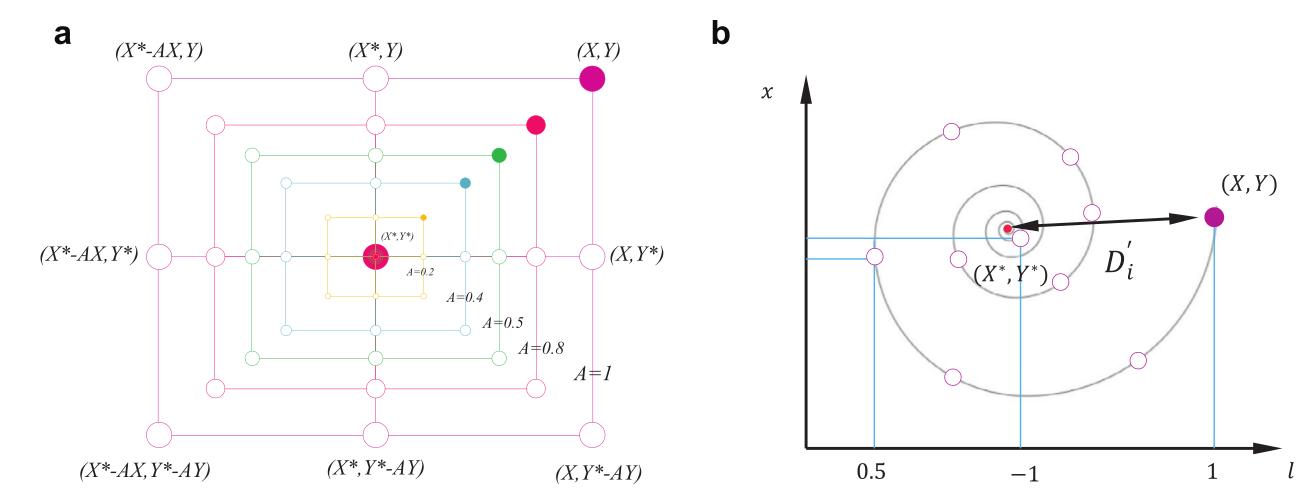
\includegraphics[scale=0.35]{./Imagenes/lineal_espiral.png}
			\caption{a) Aproximación lineal. b) Aproximación en espiral.}
		\end{figure}
		
	\subsection{Pseudocódigo del algoritmo}
	
		\begin{algorithm}[!h]
			\begin{algorithmic}[!h]
				\STATE Inicialización de la población de ballenas $X_i$ : $i=1,2,...,n$
				\STATE Se calcula el fitness de cada ballena.
				\STATE $X^*=$ la mejor de las ballenas.
				\STATE t=0
				\WHILE{t<máximo de iteraciones}
					\FOR{$X_i$ con i=1,2,...,n}
						\STATE Actualiza a,A,C,l y p (b=1).
						\IF{$p<0.5$}
							\IF{$|A|<1$}
								\STATE Actualiza la posición de la ballena $X_i$ utilizando la aproximación lineal con $X^*$
							\ELSE
								\STATE Escogemos una ballena aleatoria $X_{rand}$
								\STATE Actualiza la posición de la ballena $X_i$ utilizando la aproximación lineal con $X_{rand}$
							\ENDIF
						\ELSE
							\STATE Actualiza la posición de la ballena de forma espiral con $X^*$
						\ENDIF
					\ENDFOR
					\STATE Comprobar si alguna ballena se ha salido del espacio de búsqueda.
					\STATE Calcular el fitness de las ballenas de nuevo.
					\STATE Actualizar $X^*$
					\STATE t=t+1
				\ENDWHILE
				\RETURN $X^*$
			\end{algorithmic}
		\end{algorithm}
	
	\newpage
	
	\section{Desarrollo de mejoras}
	\label{sec:desarrolloMejoras}
	
	\subsection{Versión original}
	
	La primera aproximación al algoritmo implementado vino dada por la propia de los autores, realizada en el lenguaje Matlab y que yo tuve que adaptar a Python. Esta adaptación fue instrucción a instrucción para que el algoritmo se viera reflejado fielmente.
	
	La primera versión contiene el mismo esquema que el pseudocódigo mencionado con anterioridad pero si lo analizamos un poco mejor podemos ver que la población inicial no se genera de forma aleatoria como cabría esperar, si no que se inicializa con el vector $(0,...,0)$. Este hecho me resultó curioso cuando me di cuenta de que las funciones que se analizaban para el algoritmo tenían casi todas su mínimo en el 0. Por seguir unos propósitos más generales he decidido inicializar toda la población de forma aleatoria. En cuanto al resto del código no cambié nada puesto que quería mantener en un principio la esencia del algoritmo.
	
	\subsection{Aproximación espiral a una solución aleatoria}
	
	Para la segunda versión hice el primer cambio que comenté en la exposición de la metaheurística y que es evidente al mirar el algoritmo. Decidí meter también una búsqueda hacia una solución aleatoria si $|A|\geq 1$ en la espiral, de forma que en el primera fase del algoritmo se maximizara la búsqueda en el espacio de soluciones. Este cambio no resultó ser a mejor debido a que aunque en un principio pueda parecer lógico que el algoritmo así va a explorar más, con el tiempo y desarrollando versiones me dí cuenta de que lo que le faltaba al algoritmo no era más exploración o diversidad, si no convergencia como luego veremos.
	
	\subsection{Solis Wets}
	
	Para introducir la búsqueda local dentro del algoritmo y aportarle así un poco más de convergencia comencé implementado mi propia versión de la búsqueda local de forma parecida a cómo lo hemos hecho en las prácticas de la asignatura. Tomamos un vector de entrada y le realizamos una mutación en una de sus posiciones sumándole un valor generado por una distribución normal con $\mu = 0$ y $\sigma = 0.3$. Esto resultó ser una búsqueda local pésima que incluso era capaz de empeorar el algoritmo inicial por lo que la descarté.
	
	Tras esto acudí a los ficheros que se nos daban de ayuda, los cuales contenían una búsqueda local mucho mejor implementada en C++ pero de nuevo no me servían puesto que he realizado la implementación en Python. Acudí a la cuenta de GitHub de Daniel Molina y tras obtener su consentimiento he usado una implementación de la búsqueda local Solis Wets realizada en Python por él mismo \cite{solisWetsDanielMolina}.
	
	Esta búsqueda local se diferencia con respecto a la mía en tres aspectos. El primero de ellos es que añadido a sumar un incremento generado con una distribución normal tenemos el hecho de que se mantiene una inercia, es decir, si mejoramos el vector solución hacia una dirección concreta y nos estuvo dando éxito entonces continuaremos con una cierta inercia dirigiendo hacia allí la solución. El segundo aspecto es que si en una dirección de modificación del vector no estamos obteniendo mejoras entonces vamos a coger en la iteración siguiente justo la dirección opuesta. Por último el valor $\sigma$ de la distribución normal $\mathcal{N}(0,\sigma)$ se va incrementando o decrementando en función del número de éxitos al realizar la mejora, es decir, si superamos un umbral de éxitos incrementaremos el valor de $\sigma$ y si superamos un umbral de fallos entonces decrementaremos el valor de $\sigma$. 
	
	Con esta nueva búsqueda local realicé la tercera versión del algoritmo. La idea es que cada mil iteraciones introducimos una búsqueda local que nos va a favorecer la convergencia del algoritmo. Además para intentar mejorar lo máximo posible la solución reservo al final 1000 evaluaciones para que la búsqueda local pueda intentar mejorar el resultado del algoritmo. 
	
	Tras hacer esto de nuevo vi que la convergencia era demasiada, es decir, el algoritmo mejoraba muy rápido cuando se empleaba la búsqueda local pero en el resto del proceso no se mejoraba demasiado puesto que las ballenas acababan estando demasiado próximas entre sí. Por ello decidí meterle un esquema muy pequeño de mutación para que diversificara el proceso. En vez de realizar un movimiento en espiral decidí cambiarlo por una mutación del 20\% de la población volviendo a generarlos de forma aleatoria. Lo que conseguimos con esto es que la población vaya mejorando en términos generales, pero si entramos en la parte del algoritmo asociada a la espiral entonces mutamos para dar mas diversidad. Haciendo estos cambios como veremos posteriormente obtuve una mejora muy notoria en los resultados.
	
	\subsection{Differential Evolution}
	
    En la cuarta versión quise meter un esquema de diversidad un poco más elaborado que el de la tercera versión. Lo primero que hice fue cambiar el condicional sobre el valor aleatorio p. Ahora solo entraremos en la parte del condicional correspondiente a la espiral si $p\geq0.9$ lo cual reduce las posibilidades de entrar en la mutación.
    
    Para suplir este cambio le metí un esquema de Differential Evolution cada 10.000 iteraciones. Este esquema de Differential Evolution lo que hace es ejecutar un algoritmo de Differential Evolution durante un número de iteraciones concretas. La elección de este algoritmo vino influenciada por los buenos resultados que obtenía en todos los rankings de competiciones de algoritmos, además disponía de él de forma fácil pues lo habíamos implementado en las prácticas y por tanto sólo tenía que adaptar mi código a es de este problema. Como esquema de mutación tomé el operador Rand1 que es el que mejores resultados me dio en la práctica comparado con Current to Best 1. Cabe recordar que el esquema de mutación toma para cada individuo a mutar tres individuos aleatorios de la población y mediante un factor F obtiene el vector mutado como:
    
    $$mutado = poblacion[rand_1] + F\cdot (poblacion[rand_2]-poblacion[rand_3])$$
    
    Donde la constante F es la recomendada en las diapositivas de teoría $F=0.5.$
    
    Tras esto me di cuenta de que los resultados del algoritmo no habían mejorado todo lo que esperaba. Esta mejora está claro que desarrolla más diversidad que convergencia con respecto al esquema de la búsqueda local, por lo que decidí que, además de cambiar el umbral de p a partir del cual entramos en la mutación del 20\% de la población, iba a realizar la mutación sobre el 20\% peor y no sobre un 20\% aleatorio. Tras este cambio mejoró un poco el algoritmo.
    
    \subsection{CMAES}
    
    Llegados a este punto el algoritmo mantenía un equilibrio entre convergencia y diversidad bastante ajustado, ya que añadiendo más evaluaciones a la búsqueda local o quitándole no conseguía una mejora sustancial. Por ello se me ocurrió que más que quitar o sumar evaluaciones a la búsqueda local lo que tenía que hacer era aprovechar mejor las evaluaciones que le estaba cediendo con respecto al resto del algoritmo.
    
    Por ello decidí utilizar un algoritmo más potente como CMAES. El problema que tuve con este algoritmo fue parecido al que he relatado previamente con la búsqueda local. En primer lugar intenté acudir de nuevo a Daniel Molina para ver si tenía una versión en Python de CMAES. Esta consulta resultó satisfactoria pues sí la tenía pero al comprobar con más detalle me dí cuenta de que estaba escrita en Python2 mientras que yo estaba empleando Python3 que no tiene retrocompatibilidad. Por ello volví a preguntarle y me sugirió que usase la implementación de los propios autores que tienen disponible en su GitHub \cite{PYCMA}.
    
    Esta implementación tiene su propia sintaxis para las funciones, por lo que tuve que modificar ligeramente los ficheros de CMAES hasta que pude hacer que funcionara con mi algoritmo. El cambio realizado por tanto fue reemplazar todas las búsquedas locales por llamadas a CMAES de forma que mejorase mucho más la solución en el mismo número de evaluaciones. Este cambio le dio una mejora sustancial a los resultados aunque ya estaba acercándome a los mínimos de las funciones.
    
    \subsection{Posición aleatoria}
    
    Por último, tras revisar el algoritmo en busca de posibles mejoras empecé a prestarle atención a la fase inicial del mismo. En la fase inicial el algoritmo en vez de aproximarse hacia la mejor ballena se aproxima a una de ellas escogida de forma aleatoria. Este comportamiento puede llevar a que las ballenas se acaben agrupando entorno a ellas mismas y por tanto arruinaría la exploración. Por ello el último cambio que he realizado al algoritmo ha consistido en hacer una aproximación a un vector aleatorio en vez de a una ballena aleatoria.
    
    Esta mejora que a priori pudiera parecer un tanto trivial mejoró la exploración del algoritmo tanto que en algunos casos mejoré 1000 unidades respecto a la versión anterior.
    
	
	\section{Versión final}
	\label{sec:versionFinal}
	
	La versión final del algoritmo es la consecuencia de haber seguido la secuencia de mejoras y pruebas que he definido en la sección anterior. A continuación describiré el algoritmo en pseudocódigo:
	
	\begin{algorithm}
		\caption{Ballena(f\_obj,inf,sup,dimension,nBallenas)}
		\begin{algorithmic}
			\STATE max\_evals = $10000\cdot dimension$
			\STATE evaluaciones = 0
			\STATE Inicializo lider\_pos a un vector aleatorio con valores entre inf y sup.
			\STATE lider\_score = $\infty$
			\STATE Genero una población inicial llamada posiciones con vectores aleatorios con valores entre inf y sup.
			\STATE t = 0
			\STATE max\_iter = (0.9*max\_evals)/nBallenas
			\STATE a = 2
			\STATE Coloco en un principio el fitness de cada ballena como infinito en el vector fitness.
			\WHILE{$evaluaciones<max\_evals$}
				\IF{$t\%100==0$ and $t!=0$}
					\STATE Tomamos un 25\% de las ballenas de forma aleatoria.
					\STATE Ejecutamos CMAES sobre el 25\% elegido
					\STATE Actualizamos el vector de posiciones con las soluciones de CMAES.
					\STATE Actualizamos el vector fitness con el fitness de las soluciones.
					\STATE Sumamos a evaluaciones las evaluaciones consumidas por CMAES.
				\ENDIF
				\IF{$t\%50==0$ and $t!=0$}
					\STATE Aplico el esquema de Differential Evolution sobre el vector posiciones.
					\STATE Actualizo el vector posiciones, el vector fitness y sumo las evaluaciones consumidas por Differential Evolution.
				\ENDIF
				\STATE Comprobamos si las ballenas se han salido de los límites, actualizamos sus fitness y actualizamos lider\_pos y lider\_score si es necesario.
				\STATE Sumamos nBallenas a evaluaciones.
				\STATE $a = 2-t\cdot \frac{2}{max\_iter}$
				\FOR{i=0,...,nBallenas-1}
					\STATE Tomamos dos números aleatorios entre 0 y 1 r1 y r2.
					\STATE $A=2\cdot a\cdot r1 - a$
					\STATE $C=2\cdot r2$
					\STATE Se toma p un número aleatorio entre 0 y 1.
					\IF{$p<0.9$}
						\IF{$|A|\geq 1$}
							\STATE Tomamos X\_rand un vector aleatorio con valores en el intervalo $[inf,sup]$
							\STATE $D\_X\_rand = |C\cdot X\_rand - posiciones[i]|$
							\STATE $posiciones[i] = X\_rand-A\cdot D\_X\_rand$
						\ELSE
							\STATE $D\_lider = |C\cdot lider\_pos - posiciones[i]|$
							\STATE $posiciones[i] = lider\_pos-A\cdot D\_lider$
						\ENDIF
					\ELSE
						\STATE Tomamos la mitad peor de las ballenas y las reemplazamos por vectores aleatorios.
					\ENDIF
				\ENDFOR
			\ENDWHILE
			\STATE Comprobamos si las ballenas se han salido de los límites, actualizamos sus fitness y actualizamos lider\_pos y lider\_score si es necesario.
			\STATE Aplicamos CMAES sobre lider\_pos.
			\RETURN lider\_pos, lider\_score
		\end{algorithmic}
	\end{algorithm}

	He tomado como máximo de evaluaciones 10.000 por la dimensión, al igual que venía especificado para la competición CEC2014.

	El algoritmo recibe como parámetros la función objetivo, el extremo inferior del espacio de búsqueda, el extremo superior, la dimensión del problema y el número de ballenas que se quiere que tenga la población, por defecto 50.
	
	Para definir el máximo de iteraciones tomo el 90\% de las mismas para reservar un 10\% para que cuando llegue al final del algoritmo pueda ejecutar CMAES sobre la mejor de las ballenas con dicho 10\% de las iteraciones máximas.
	
	\section{Resultados}
	\label{sec:resultados}
	
	En primer lugar vamos a estudiar cómo ha evolucionado el esquema de soluciones en cuanto a resultados para comprobar que en términos generales el algoritmo ha mejorado de forma muy notable. En un principio el algoritmo obtuvo unos resultados muy lejanos de los óptimos. El valor óptimo de la función en cada caso es $i\cdot 100$ donde i corresponde al número de la función.
	
	Teniendo en cuenta esto los errores y resultados obtenidos para las 20 funciones con la implementación inicial fueron:
	
	\begin{figure}[!h]
		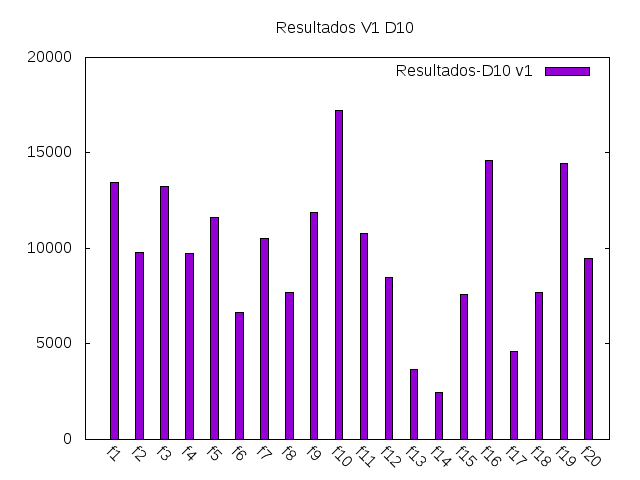
\includegraphics[scale=0.5]{../Algoritmo/resultados/Imagenes/Resultados/resultados_v1_d10.png}
		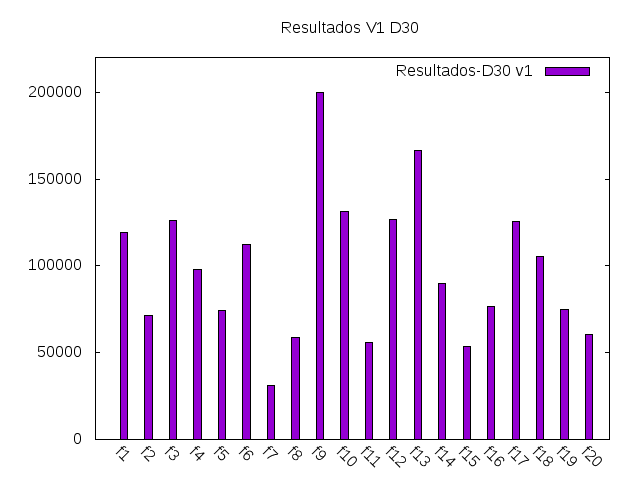
\includegraphics[scale=0.5]{../Algoritmo/resultados/Imagenes/Resultados/resultados_v1_d30.png}
		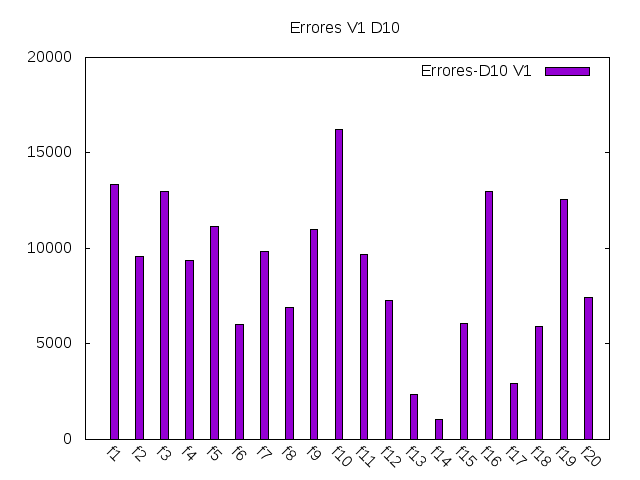
\includegraphics[scale=0.5]{../Algoritmo/resultados/Imagenes/Errores/errores_v1_d10.png}
		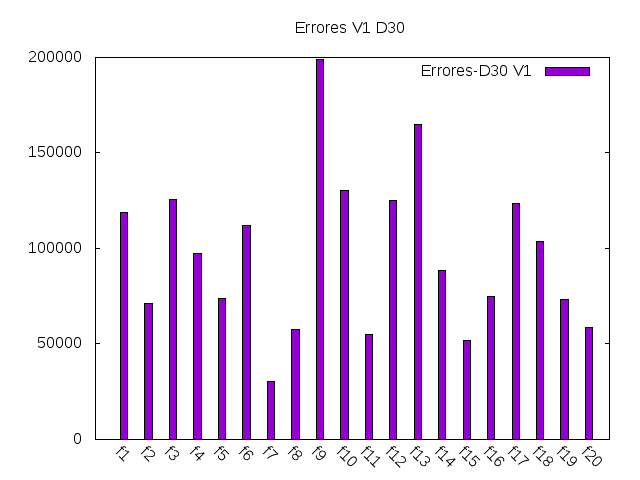
\includegraphics[scale=0.5]{../Algoritmo/resultados/Imagenes/Errores/errores_v1_d30.png}
		\caption{Resultados y errores de la primera versión}
	\end{figure}

	Si nos damos cuenta para dimensión 10 los resultados obtenidos llegan a estar incluso cerca de 17.500 y para dimensión 30 cerca de los 200.000 lo que está muy alejado de los valores óptimos de las funciones. 
	
	Este comportamiento me resultó raro ya que en el paper se comparaba este algoritmo en problemas de minimización de funciones con otros muchos algoritmos y ganaba en casi todos los casos. Tras comprobar bien la implementación y las funciones vi que los mínimos de las funciones estaban casi todos en el punto 0 del espacio o muy cercano a el y que las ballenas iniciales se inicializaban todas en la posición 0. Este hecho puede llevar a pensar que los resultados estén condicionados por la localización del óptimo en las funciones ya que con la misma implementación pero cambiando el óptimo de posición en las funciones que se quieren minimizar ya no obtenemos unos resultados tan buenos.
	
	Si seguimos comparando podemos ver que en la versión tres mejoramos los resultados un poco con respecto a la primera:
	
	\begin{figure}[!h]
		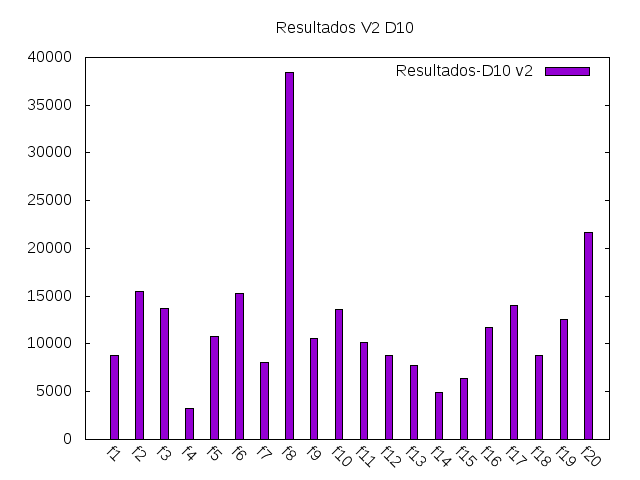
\includegraphics[scale=0.5]{../Algoritmo/resultados/Imagenes/Resultados/resultados_v2_d10.png}
		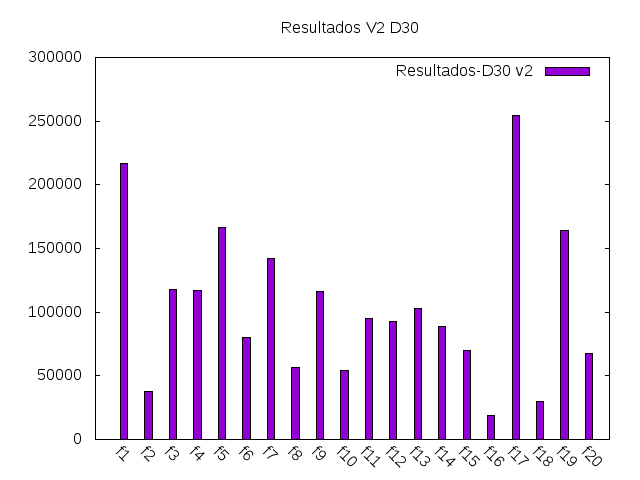
\includegraphics[scale=0.5]{../Algoritmo/resultados/Imagenes/Resultados/resultados_v2_d30.png}
		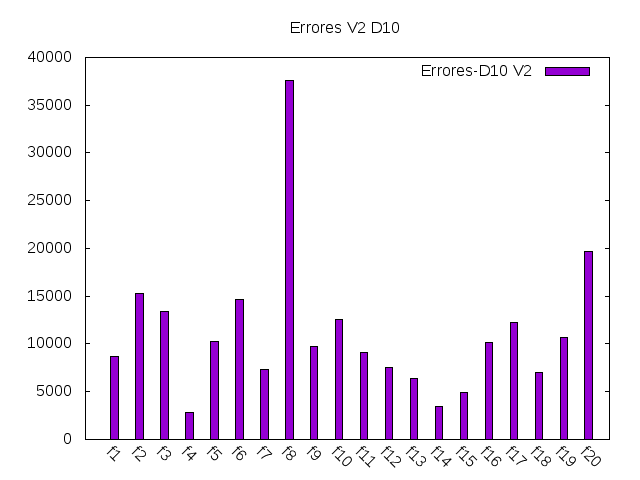
\includegraphics[scale=0.5]{../Algoritmo/resultados/Imagenes/Errores/errores_v2_d10.png}
		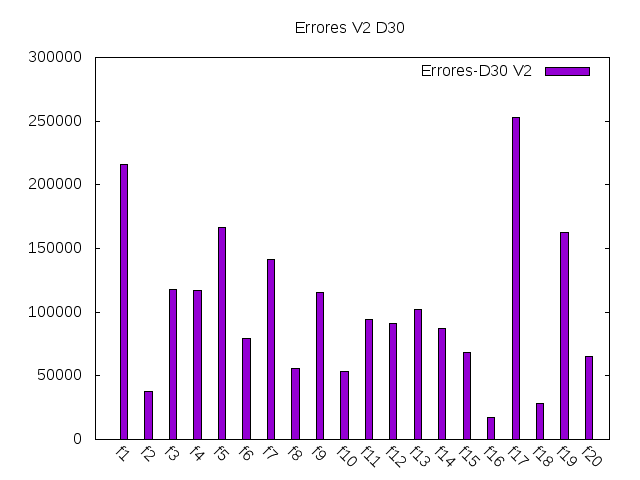
\includegraphics[scale=0.5]{../Algoritmo/resultados/Imagenes/Errores/errores_v2_d30.png}
		\caption{Resultados y errores de la segunda versión}
	\end{figure}

	Podemos observar que la mejora ha sido en términos generales buena, pero aún así seguimos encontrando funciones que destacan por dar unos valores mucho peores que el resto. Cabe destacar que en esta versión encontramos más diversidad y menor convergencia, cosa que se invertirá en la próxima versión:
	
	\begin{figure}[!h]
		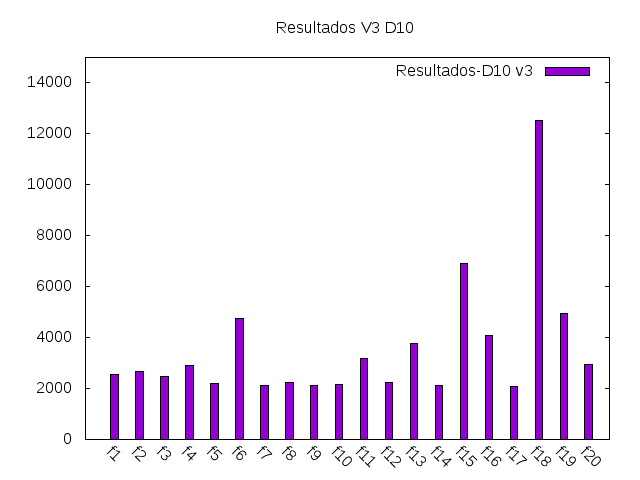
\includegraphics[scale=0.5]{../Algoritmo/resultados/Imagenes/Resultados/resultados_v3_d10.png}
		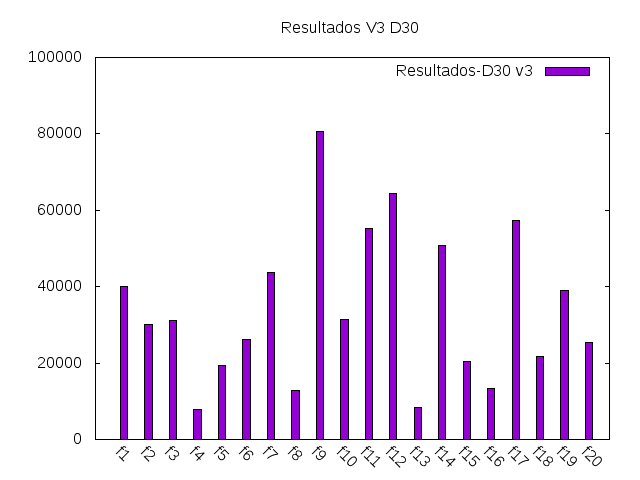
\includegraphics[scale=0.5]{../Algoritmo/resultados/Imagenes/Resultados/resultados_v3_d30.png}
		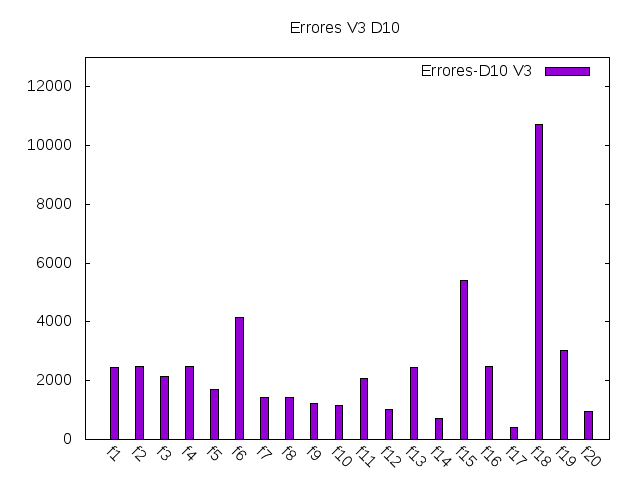
\includegraphics[scale=0.5]{../Algoritmo/resultados/Imagenes/Errores/errores_v3_d10.png}
		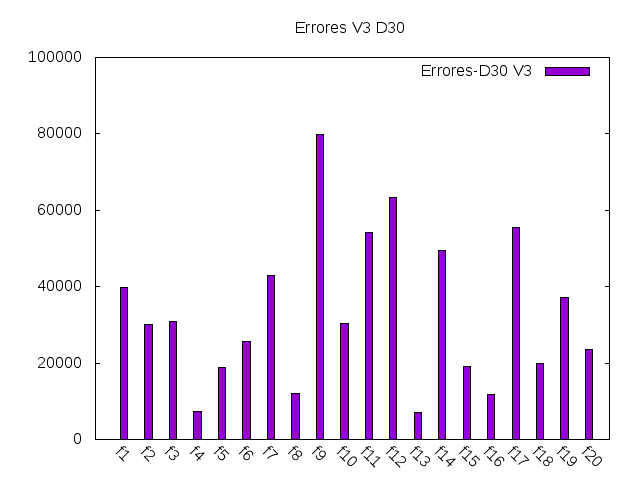
\includegraphics[scale=0.5]{../Algoritmo/resultados/Imagenes/Errores/errores_v3_d30.png}
		\caption{Resultados y errores de la tercera versión}
	\end{figure}

	\newpage

	En esta versión sí notamos una escalada realmente buena en los resultados que nos han mejorado enormemente en la versión de dimensión 10 pero aún más en dimensión 30 donde se han llegado a reducir a la mitad. Tras este cambio como comenté en la explicación de las versiones introduje más diversidad con un esquema de Differential Evolution lo cual condujo al algoritmo a la primera mejora realmente sustancial:
	
	\begin{figure}[!h]
		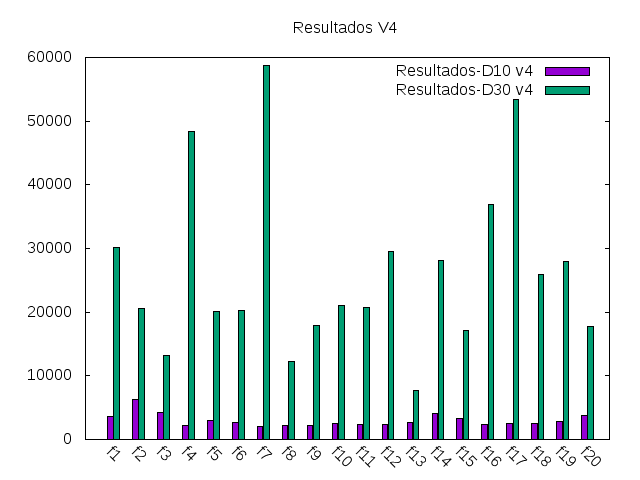
\includegraphics[scale=0.5]{../Algoritmo/resultados/Imagenes/Resultados/resultados_v4.png}
		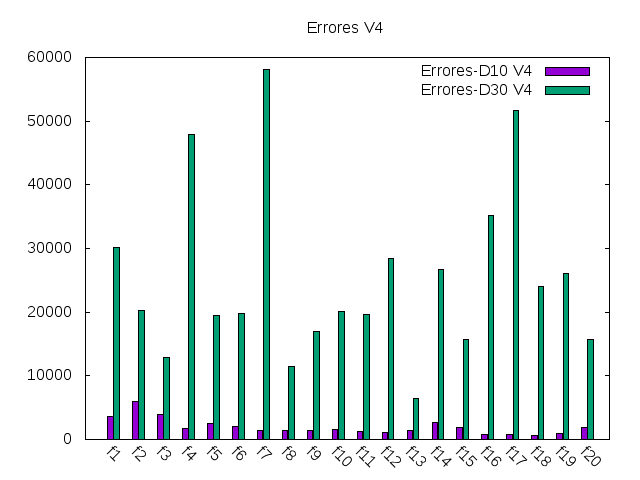
\includegraphics[scale=0.5]{../Algoritmo/resultados/Imagenes/Errores/errores_v4.png}
		\caption{Resultados y errores de la cuarta versión}
	\end{figure}

	\newpage

	En esta versión es la primera en la que los resultados generales de ambas dimensiones bajan lo suficiente como para poder representarlas las dos juntas. Esta mejora nos indica que en el algoritmo previo habíamos excedido los esfuerzos en convergencia y estábamos equilibrando mal la diversidad. 
	
	La cuarta versión tuvo como cambio importante la introducción de CMAES:
	
	\begin{figure}[!h]
		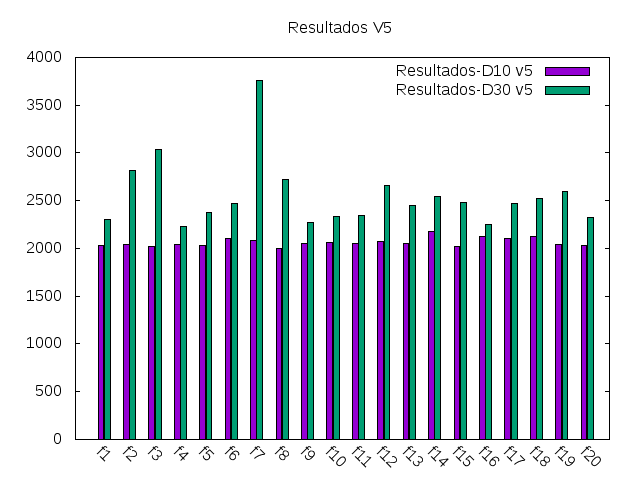
\includegraphics[scale=0.5]{../Algoritmo/resultados/Imagenes/Resultados/resultados_v5.png}
		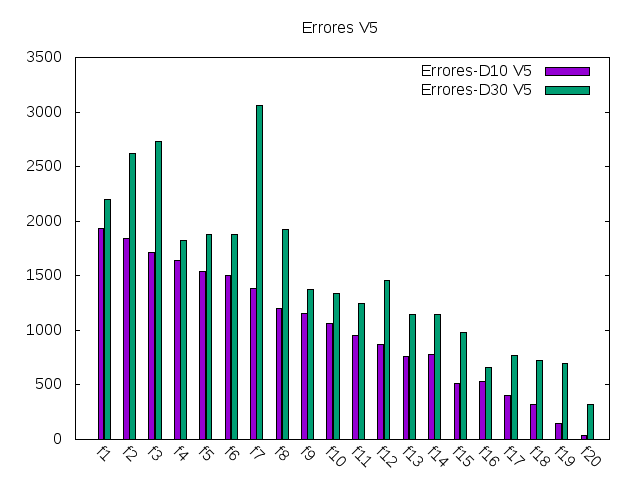
\includegraphics[scale=0.5]{../Algoritmo/resultados/Imagenes/Errores/errores_v5.png}
		\caption{Resultados y errores de la quinta versión}
	\end{figure}

	Aquí observamos la gran potencia de CMAES que nos ha conseguido bajar los resultados de los dos algoritmos por debajo de 4.000 lo cual es un resultado muy diferente al obtenido en la primera versión. Por último los resultados y errores cometidos tras incorporar la última mejora finales han sido:
	
	\newpage
	
	\begin{figure}[!h]
		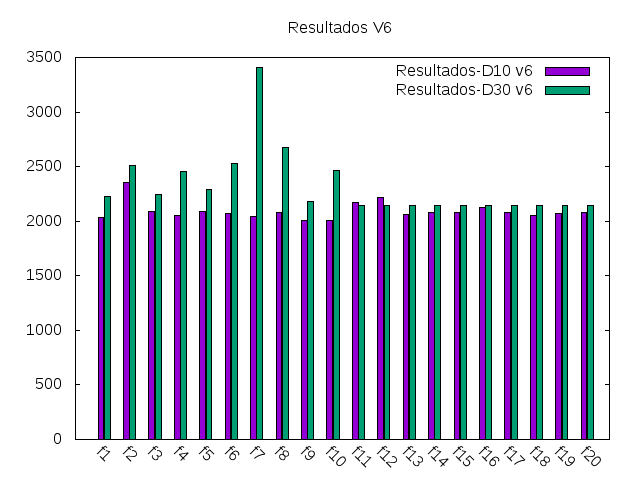
\includegraphics[scale=0.5]{../Algoritmo/resultados/Imagenes/Resultados/resultados_v6.png}
		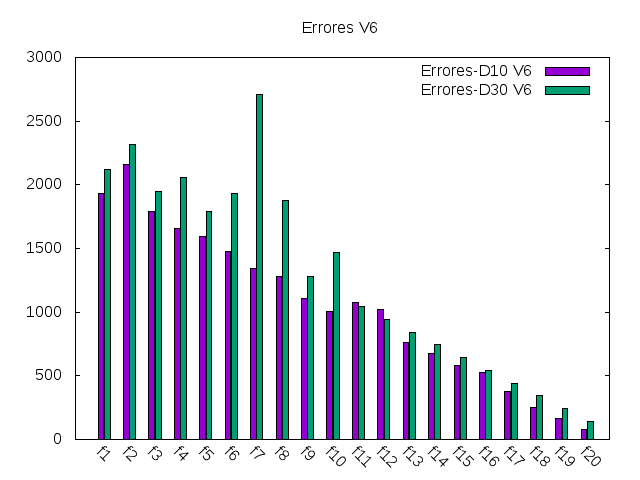
\includegraphics[scale=0.5]{../Algoritmo/resultados/Imagenes/Errores/errores_v6.png}
		\caption{Resultados y errores de la sexta versión}
	\end{figure}

	Así mismo podemos ver la progresión del algoritmo, esto es, vamos a ver cómo evolucionan las mejores ballenas en cada iteración del algoritmo y vamos a analizarlo:
	
	\begin{figure}[!h]
		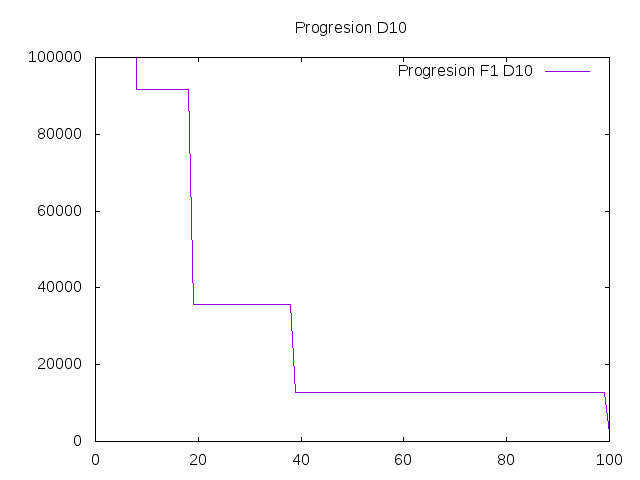
\includegraphics[scale=0.5]{../Algoritmo/resultados/Imagenes/Progresion/progresion_mejores_10.png}
		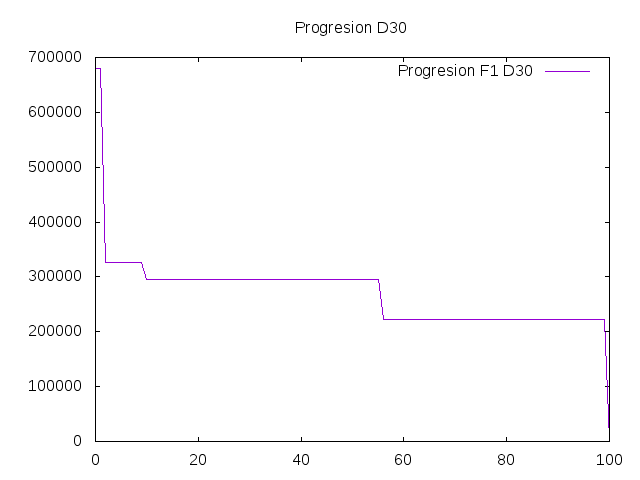
\includegraphics[scale=0.5]{../Algoritmo/resultados/Imagenes/Progresion/progresion_mejores_30.png}
		\caption{Progresión de las mejores ballenas en la versión final.}
	\end{figure}

	En estas progresiones se puede observar cómo las mejores ballenas cambian sólo en los múltiplos de 10. Es en este momento cuando aplicamos CMAES y el esquema de Differential Evolution, es decir, realmente sólo mejoran las ballenas sustancialmente cuando aplicamos los dos algoritmos auxiliares. Esto nos deja como conclusión obvia que el esquema de movimiento dado por el algoritmo inicial no es realmente eficaz, ya que no consigue mejoras notables sobre las ballenas ni obtiene buenos resultados por sí solo.
	
	Este esquema de progresión fue muy parecido sobre todas las funciones, por lo que sólo he decidido poner el de la primera función en ambas dimensiones como ejemplo concreto.
	
	\subsection{Comparativa con el resto de algoritmos}
	
	Para la comparativa vamos a hacer 3 tablas diferentes: una tabla con los algoritmos de la competición CEC2014, otra con la tabla de Tanabe y por último una comparando con los dos algoritmos de Differential Evolution implementados por Daniel Molina. Estas tablas representan el error cometido en cada una de las funciones y el error acumulado de las mismas.
	
	\begin{table}[!h]
		\centering
		\resizebox{\textwidth}{!}{
			\begin{tabular}{ | l | l | l | l | l | l | l | l | l | l | l | l | l | }
				\hline
				\textbf{\underline{Funciones}} & \textbf{\underline{CoDE}} & \underline{\textbf{D-SHADE}} & \underline{\textbf{EPSDE}} & \underline{\textbf{JADE}} & \underline{\textbf{L-SHADE}} & \underline{\textbf{NBIPOP-aCMA-ES}} & \underline{\textbf{SHADE11}} & \underline{\textbf{SaDE}} & \underline{\textbf{dynNP-jDE}} & \underline{\textbf{iCMAES-ILS}} & \underline{\textbf{WOA}} \\ \hline
				F1 & 0 & 0 & 0 & 0 & 0 & 0 & 0 & 2.5523 & 2.1693E-7 & 0 & 1932.1809 \\ \hline
				F2 & 0 & 0 & 0 & 0 & 0 & 0 & 0 & 0 & 0 & 0 & 2155.8268 \\ \hline
				F3 & 0 & 0 & 0 & 6.1659E-3 & 0 & 0 & 0 & 0 & 0 & 0 & 1790.9763 \\ \hline
				F4 & 10.4826 & 30.7734 & 0 & 27.6186 & 29.4095 & 2.8198 & 29.4945 & 18.0850 & 3.3229 & 14.3852 & 1655.7516 \\ \hline
				F5 & 18.4489 & 17.7268 & 20.0499 & 17.2676 & 14.1455 & 18.0702 & 18.0061 & 15.7840 & 15.9500 & 14.6543 & 1591.2193 \\ \hline
				F6 & 1.6525E-6 & 0 & 3.0415 & 0.1755 & 1.7540E-2 & 0.3305 & 0 & 0 & 0 & 0 & 1474.9728 \\ \hline
				F7 & 3.7590E-2 & 5.3139E-3 & 1.7573E-2 & 1.1861E-2 & 3.04292E-3 & 0 & 9.7818E-3 & 7.2428E-3 & 4.9691E-3 & 0 & 1342.4297 \\ \hline
				F8 & 0 & 0 & 0 & 0 & 0 & 3.6972 & 0 & 0 & 0 & 0.2536 & 1277.5693 \\ \hline
				F9 & 3.8822 & 3.0826 & 3.6887 & 3.5070 & 2.3445 & 0.3262 & 3.1407 & 3.5837 & 3.8578 & 9.7548E-2 & 1106.6753 \\ \hline
				F10 & 3.5513E-2 & 4.8983E-2 & 4.4085E-2 & 6.1229E-3 & 8.5721E-3 & 91.6179 & 1.2245E-2 & 1.9593E-2 & 2.4491E-3 & 122.0401 & 1007.0534 \\ \hline
				F11 & 75.9702 & 54.9344 & 323.1316 & 83.6964 & 32.0558 & 116.8327 & 63.1801 & 196.4226 & 136.2141 & 8.5850 & 1073.7122 \\ \hline
				F12 & 4.3383E-2 & 5.2908E-2 & 0.3210 & 0.2501 & 6.8167E-2 & 1.0083E-2 & 0.1364 & 0.4350 & 0.3111 & 6.5009E-2 & 1020.3847 \\ \hline
				F13 & 7.9798E-2 & 4.8919E-2 & 0.1223 & 8.3967E-2 & 5.1561E-2 & 1.0894E-2 & 7.3996E-2 & 0.1252 & 0.1189 & 9.1148E-3 & 761.6723 \\ \hline
				F14 & 0.1071 & 9.0096E-2 & 0.1363 & 0.1105 & 8.1361E-2 & 0.2824 & 0.1055 & 0.1857 & 0.1352 & 0.1545 & 675.8475 \\ \hline
				F15 & 0.6523 & 0.4027 & 0.7538 & 0.5782 & 0.3660 & 0.5467 & 0.5051 & 0.7903 & 0.7815 & 0.7233 & 580.7508 \\ \hline
				F16 & 1.1291 & 1.3390 & 2.5412 & 1.6508 & 1.2407 & 2.5295 & 1.5571 & 1.9669 & 1.5944 & 1.9070 & 524.9302 \\ \hline
				F17 & 2.6621 & 3.3813 & 53.2895 & 30.9109 & 0.9766 & 38.8964 & 1.5576 & 28.3335 & 2.6228 & 21.0348 & 378.5809 \\ \hline
				F18 & 0.4305 & 0.4749 & 1.1971 & 0.2387 & 0.2440 & 3.5766 & 0.2369 & 1.6451 & 0.4409 & 0.5259 & 250.5374 \\ \hline
				F19 & 7.4471E-2 & 0.2050 & 1.4319 & 0.2549 & 7.7300E-2 & 0.8276 & 0.1916 & 6.6889E-2 & 0.1218 & 0.7076 & 166.1558 \\ \hline
				F20 & 2.3911E-2 & 0.2733 & 0.1650 & 0.3240 & 0.1848 & 1.3167 & 0.2433 & 0.1076 & 4.1478E-2 & 0.8040 & 78.7133 \\ \hline
				Suma & 114.0602 & 112.8402 & 409.9321 & 166.6920 & 81.2756 & 281.6920 & 118.4516 & 270.1111 & 165.5208 & 185.9477 & 20845.9416 \\ \hline
			\end{tabular}
		}
		\label{tablaTANABE-D10}
		\caption{Resultados comparados Tanabe dimensión 10}
	\end{table}


	\begin{table}[!h]
		\centering
		\resizebox{\textwidth}{!}{
			\begin{tabular}{ | l | l | l | l | l | l | l | l | l | l | l | l | l | l | l | l | l | l | l | }
				\hline
				\underline{\textbf{Funciones}} & \underline{\textbf{CMLSP}} & \underline{\textbf{FCDE}} & \underline{\textbf{FERDE}} & \underline{\textbf{FWA-DM}} & \underline{\textbf{GaAPADE}} & \underline{\textbf{MVMO}} & \underline{\textbf{NRGA}} & \underline{\textbf{OptBees}} & \underline{\textbf{POBL\_ADE}} & \underline{\textbf{RSDE}} & \underline{\textbf{SOO}} & \underline{\textbf{SOO+BOBYQA}} & \underline{\textbf{UMOEAS}} & \underline{\textbf{b3e3pbest}} & \underline{\textbf{rmalschcma}} & \underline{\textbf{WOA}}  \\ \hline
				F1 & 1.7687E-7 & 1150612.9411 & 5234091.4243 & 5013.0489 & 0 & 4.9540E-4 & 27904.5013 & 784.1906 & 16226.5696 & 0 & 8810740 & 4569.72 & 0 & 2626511.6879 & 0 & 1932.1809 \\ \hline
				F2 & 1.1145E-15 & 16034575.5021 & 138042857.4263 & 1.3418E-4 & 0 & 7.0984E-9 & 914.6605 & 9.8826E-3 & 2273.0552 & 0 & 6.3429 & 3.6000E-2 & 0 & 224053205.9407 & 0 & 2155.8268 \\ \hline
				F3 & 1.0555E-4 & 1234.9883 & 4545.6467 & 1.8773E-9 & 0 & 9.8596E-11 & 1516.8063 & 0.9213 & 5.7445E-4 & 0 & 6643.6700 & 5842.9200 & 0 & 4305.3999 & 1.0254E-7 & 1790.9763 \\ \hline
				F4 & 3.3437E-15 & 41.9776 & 48.4558 & 1.4132 & 30.6882 & 9.5456 & 15.4355 & 2.6908 & 25.5082 & 2.8109 & 0.6779 & 0 & 0 & 52.5332 & 8.5007E-2 & 1655.7516 \\ \hline
				F5 & 16.8630 & 20.3811 & 20.0914 & 20.0272 & 19.6767 & 16.5805 & 19.6068 & 19.9999 & 19.0870 & 19.2163 & 20 & 20 & 16.8309 & 20.2129 & 13.6519 & 1591.2193 \\ \hline
				F6 & 6.2010E-2 & 5.3279 & 3.4732 & 0.7063 & 0.1483 & 3.4445E-3 & 2.4498 & 3.0166 & 1.0394 & 5.2908E-2 & 1.9999E-3 & 1.9999E-3 & 0 & 2.7907 & 1.4786E-4 & 1474.9728 \\ \hline
				F7 & 0 & 0.8226 & 2.1930 & 9.4799E-2 & 3.1634E-3 & 1.8583E-2 & 0.2030 & 0.1561 & 0.1626 & 3.5496E-2 & 4.8999E-2 & 4.8999E-2 & 0 & 3.3068 & 0 & 1342.4297 \\ \hline
				F8 & 2.0706 & 14.2271 & 9.7698 & 0.2536 & 0 & 6.6874E-15 & 5.5847 & 1.1591E-13 & 7.8088 & 0.6608 & 18.904 & 18.904 & 0 & 13.2486 & 0 & 1277.5693 \\ \hline
				F9 & 1.6585 & 35.7932 & 18.7457 & 6.0084 & 3.3790 & 3.4921 & 8.6936 & 20.8355 & 7.6307 & 8.5224 & 8.9550 & 8.9550 & 2.7254 & 21.0368 & 3.3165 & 1106.6753 \\ \hline
				F10 & 196.1156 & 488.5916 & 151.5188 & 1.5926 & 0.1517 & 2.1369 & 119.4300 & 219.2256 & 153.4006 & 68.4415 & 130.3900 & 130.3900 & 0.3738 & 330.8470 & 7.6779 & 1007.0534 \\ \hline
				F11 & 152.9957 & 976.2717 & 537.6226 & 372.2404 & 183.1153 & 96.2760 & 575.9476 & 392.7479 & 208.2013 & 290.6418 & 349.0499 & 349.0499 & 144.0443 & 782.9861 & 20.1349 & 1073.7122 \\ \hline
				F12 & 3.0265E-2 & 1.1285 & 0.6297 & 4.2494E-2 & 0.1402 & 4.2227E-2 & 0.1241 & 0.1303 & 0.2694 & 0.2206 & 0 & 0 & 0 & 0.8030 & 1.6464E-2 & 1020.3847 \\ \hline
				F13 & 2.7249E-2 & 0.3054 & 0.3352 & 0.1206 & 6.0087E-2 & 3.5533E-2 & 0.1576 & 0.4161 & 0.1311 & 0.1276 & 2.9999E-2 & 2.9999E-2 & 9.4357E-3 & 0.3124 & 3.2923E-2 & 761.6723 \\ \hline
				F14 & 0.1891 & 0.3380 & 1.0070 & 0.2139 & 9.4239E-2 & 8.9059E-2 & 0.2537 & 0.3686 & 0.2602 & 0.1359 & 0.13 & 0.13 & 0.11 & 0.6884 & 0.1264 & 675.8475 \\ \hline
				F15 & 0.8966 & 5.7665 & 19.1365 & 0.7748 & 0.6056 & 0.4346 & 1.0218 & 2.4388 & 0.7118 & 0.9830 & 0.44 & 0.42 & 0.6666 & 47.0112 & 0.4714 & 580.7508 \\ \hline
				F16 & 1.5545 & 3.5059 & 2.9222 & 1.7570 & 1.9771 & 1.4485 & 2.7469 & 2.6395 & 1.4090 & 2.2333 & 2.5199 & 2.5199 & 1.5302 & 2.8261 & 1.0541 & 524.9302 \\ \hline
				F17 & 312.7451 & 1765.6175 & 314731.7368 & 254.5371 & 9.9143 & 9.3566 & 16074.9090 & 684.3998 & 257.2398 & 47.7016 & 3122910 & 422.5699 & 8.4768 & 101237.2321 & 78.3384 & 378.5809 \\ \hline
				F18 & 30.8529 & 309.4347 & 234239.5987 & 25.1581 & 0.2229 & 0.7825 & 7419.7540 & 33.5042 & 33.1615 & 1.9961 & 12932.0999 & 3951.6199 & 0.7840 & 225413.4875 & 5.2207 & 250.5374 \\ \hline
				F19 & 1.2511 & 1.6141 & 2.0320 & 1.2991 & 0.2565 & 0.1583 & 2.0933 & 0.9330 & 2.0878 & 1.0302 & 0.5499 & 0.5499 & 0.1999 & 2.3744 & 7.6607E-2 & 166.1558 \\ \hline
				F20 & 19.9406 & 235.2391 & 407578.2439 & 13.3705 & 0.4315 & 0.3125 & 1719.1836 & 8.9575 & 12.5894 & 0.7214 & 9364.2 & 6925.0999 & 0.3705 & 5688.9166 & 8.0566 & 78.7133 \\ \hline
				Suma & 737.2535 & 17190329.7749 & 144238862.0105 & 5712.6597 & 250.8654 & 140.7138 & 56303.5640 & 2177.5830 & 19230.3250 & 445.5327 & 11963128.011 & 22242.9659 & 176.1225 & 227017643.6434 & 138.2605 & 20845.9416 \\ \hline
			\end{tabular}
		}
		\label{tablaCEC2014-D10}
		\caption{Resultados comparados CEC2014 dimensión 10}
	\end{table}

	\begin{table}[!h]
		\centering
		\resizebox{200pt}{!}{
			\begin{tabular}{ | l | l | l | l | l | l | l | l | l | l | l | l | l | l | l | l | l | l | l | }
				\hline
				\underline{\textbf{Funciones}} & \underline{\textbf{DEBin}} & \underline{\textbf{DEexp}} & \underline{\textbf{WOA}} \\ \hline
				F1 & 0 & 0 & 1932.1809 \\ \hline
				F2 & 0 & 0 & 2155.8268 \\ \hline
				F3 & 0 & 0 & 1790.9763 \\ \hline
				F4 & 21.5699 & 21.9087 & 1655.7516 \\ \hline
				F5 & 20.2184 & 20.1419 & 1591.2193 \\ \hline
				F6 & 0.58381 & 0.1843 & 1474.9728 \\ \hline
				F7 & 3.6599E-2 & 3.5799E-2 & 1342.4297 \\ \hline
				F8 & 4.3523 & 3.9800E-2 & 1277.5693 \\ \hline
				F9 & 11.9865 & 8.7932 & 1106.6753 \\ \hline
				F10 & 51.9530 & 11.4780 & 1007.0534 \\ \hline
				F11 & 444.452 & 555.4320 & 1073.7122 \\ \hline
				F12 & 0.4259 & 0.4390 & 1020.3847 \\ \hline
				F13 & 0.1140 & 0.1119 & 761.6723 \\ \hline
				F14 & 0.1760 & 0.1630 & 675.8475 \\ \hline
				F15 & 1.7739 & 1.2409 & 580.7508 \\ \hline
				F16 & 2.3389 & 2.3529 & 524.9302 \\ \hline
				F17 & 16.4060 & 8.4899 & 378.5809 \\ \hline
				F18 & 0.5399 & 0.5540 & 250.5374 \\ \hline
				F19 & 0.3109 & 0.4529 & 166.1558 \\ \hline
				F20 & 0.2040 & 6.5999E-2 & 78.7133 \\ \hline
				Suma & 577.4427 & 631.8847 & 20845.9416 \\ \hline
			\end{tabular}
		}
		\label{tablaDM-D10}
		\caption{Resultados comparados Daniel Molina dimensión 10}
	\end{table}

	\newpage
	\clearpage

	\begin{table}[!h]
		\centering
		\resizebox{\textwidth}{!}{
			\begin{tabular}{ | l | l | l | l | l | l | l | l | l | l | l | l | l | }
				\hline
				\textbf{\underline{Funciones}} & \textbf{\underline{CoDE}} & \underline{\textbf{D-SHADE}} & \underline{\textbf{EPSDE}} & \underline{\textbf{JADE}} & \underline{\textbf{L-SHADE}} & \underline{\textbf{NBIPOP-aCMA-ES}} & \underline{\textbf{SHADE11}} & \underline{\textbf{SaDE}} & \underline{\textbf{dynNP-jDE}} & \underline{\textbf{iCMAES-ILS}} & \underline{\textbf{WOA}} \\ \hline
				F1 & 26331.8869 & 5.0418E-3 & 24161.6368 & 447.8196 & 0 & 0 & 481.3446 & 298971.3391 & 46510.1940 & 0 & 2122.5485 \\ \hline
				F2 & 0 & 0 & 0 & 0 & 0 & 0 & 0 & 0 & 0 & 0 & 2312.8342 \\ \hline
				F3 & 0 & 0 & 0 & 5.62918E-4 & 0 & 0 & 0 & 14.2579 & 0 & 0 & 1946.9675 \\ \hline
				F4 & 2.5174 & 5.0271E-9 & 3.2126 & 0 & 0 & 0 & 0 & 37.1840 & 2.0351 & 0 & 2059.1074 \\ \hline
				F5 & 20.0638 & 20.0141 & 20.3465 & 20.2871 & 20.1146 & 20.5171 & 20.1010 & 20.5356 & 20.2912 & 19.9999 & 1790.3438 \\ \hline
				F6 & 1.9890 & 5.9243E-2 & 18.8932 & 9.4228 & 1.3843E-7 & 0.7135 & 0.5289 & 5.4599 & 1.1962 & 3.9953E-3 & 1931.7902 \\ \hline
				F7 & 1.4502E-4 & 0 & 2.0760E-3 & 0 & 0 & 0 & 4.8332E-4 & 1.2333E-2 & 0 & 0 & 2705.6641 \\ \hline
				F8 & 0 & 0 & 0 & 0 & 0 & 9.9779 & 0 & 7.8036E-2 & 0 & 2.4170 & 1874.7347 \\ \hline
				F9 & 40.3709 & 8.7033 & 44.3622 & 26.1659 & 6.7848 & 3.2411 & 15.8317 & 38.1205 & 33.9322 & 2.5650 & 1281.2102 \\ \hline
				F10 & 0.5001 & 3.5106E-2 & 0.2013 & 5.3068E-3 & 1.6328E-2 & 636.0031 & 1.2658E-2 & 0.2691 & 4.0822E-3 & 145.0062 & 1466.8371 \\ \hline
				F11 & 1951.2929 & 1303.9673 & 3564.6341 & 1639.9441 & 1229.4790 & 731.4947 & 1396.9447 & 3147.4624 & 1953.7416 & 73.8476 & 1042.3630 \\ \hline
				F12 & 5.9988E-2 & 9.6652E-2 & 0.5251 & 0.2711 & 0.1605 & 1.3220E-2 & 0.1622 & 0.7941 & 0.3620 & 2.8288E-2 & 942.3630 \\ \hline
				F13 & 0.2312 & 0.1343 & 0.2429 & 0.2202 & 0.1241 & 3.8913E-2 & 0.2040 & 0.2515 & 0.2531 & 2.9511E-2 & 842.3630 \\ \hline
				F14 & 0.2388 & 0.2317 & 0.2781 & 0.2339 & 0.2417 & 0.3278 & 0.2246 & 0.2285 & 0.2656 & 0.1698 & 742.3630 \\ \hline
				F15 & 3.1752 & 1.8918 & 5.6692 & 3.0979 & 2.1463 & 2.1358 & 2.5641 & 4.1410 & 4.7558 & 2.5110 & 642.3630 \\ \hline
				F16 & 9.2624 & 8.5185 & 11.1464 & 9.3698 & 8.4990 & 10.6241 & 9.1477 & 10.9108 & 9.2242 & 10.8701 & 542.3630 \\ \hline
				F17 & 1452.9858 & 210.3202 & 46053.1842 & 9673.3938 & 187.5081 & 852.2059 & 1058.9064 & 11530.6982 & 957.7013 & 1046.7457 & 442.3630 \\ \hline
				F18 & 13.4426 & 10.3642 & 331.8819 & 358.0523 & 5.9100 & 115.3533 & 49.8746 & 443.8338 & 21.0203 & 96.0895 & 342.3630 \\ \hline
				F19 & 2.7041 & 3.5275 & 13.3001 & 4.4373 & 3.6817 & 5.6999 & 4.3057 & 4.0013 & 3.9067 & 6.4564 & 242.3630 \\ \hline
				F20 & 10.9130 & 4.2016 & 50.0424 & 2885.3663 & 3.0818 & 24.03930 & 12.6424 & 124.5428 & 8.5281 & 33.5459 & 142.3630 \\ \hline
				Suma & 29841.6352 & 1572.0709 & 74279.5599 & 15078.0887 & 1467.7486 & 2412.3861 & 3052.7963 & 314354.1218 & 49527.4122 & 1440.2863 & 25415.6688 \\ \hline
			\end{tabular}
		}
		\label{tablaTANABE-D30}
		\caption{Resultados comparados Tanabe dimensión 30}
	\end{table}
	
	
	\begin{table}[!h]
		\centering
		\resizebox{\textwidth}{!}{
			\begin{tabular}{ | l | l | l | l | l | l | l | l | l | l | l | l | l | l | l | l | l | l | l | }
				\hline
				\underline{\textbf{Funciones}} & \underline{\textbf{CMLSP}} & \underline{\textbf{FCDE}} & \underline{\textbf{FERDE}} & \underline{\textbf{FWA-DM}} & \underline{\textbf{GaAPADE}} & \underline{\textbf{MVMO}} & \underline{\textbf{NRGA}} & \underline{\textbf{OptBees}} & \underline{\textbf{POBL\_ADE}} & \underline{\textbf{RSDE}} & \underline{\textbf{SOO}} & \underline{\textbf{SOO+BOBYQA}} & \underline{\textbf{UMOEAS}} & \underline{\textbf{b3e3pbest}} & \underline{\textbf{rmalschcma}} & \underline{\textbf{WOA}}  \\ \hline
				F1 & 3.9810E-10 & 39737210.0987 & 74247962.7037 & 276356.8617 & 1.0031E-14 & 1.0664E-3 & 574302.4960 & 85681.0783 & 15954.8321 & 1500.2888 & 215525900 & 2674850 & 0 & 13225062.5980 & 0 & 2122.5485 \\ \hline
				F2 & 0 & 1759112643.3250 & 3467117007.8945 & 1.0754E-16 & 1.6718E-15 & 2.3800E-5 & 9276.2813 & 3.3175E-12 & 313.6770 & 1.1914E-9 & 31387 & 99.6109 & 0 & 517280687.2460 & 0 & 2312.8342 \\ \hline
				F3 & 1.2335E-8 & 9119.3176 & 13921.8438 & 4.4236E-16 & 2.2291E-15 & 1.1057E-3 & 4581.8338 & 8.4136E-3 & 6.4296E-10 & 4.7433E-2 & 10810.2 & 7840.39 & 0 & 5609.1629 & 26.1949 & 1946.9675 \\ \hline
				F4 & 2.1734E-6 & 196.6229 & 489.4935 & 20.3624 & 2.8276E-12 & 4.3802E-13 & 80.5810 & 12.5634 & 63.4483 & 3.0517 & 109.3459 & 36.755 & 0 & 63.4242 & 0 & 2059.1074 \\ \hline
				F5 & 19.9989 & 20.9567 & 20.1969 & 20.5059 & 20.0022 & 19.9995 & 20.0001 & 19.9999 & 20.6376 & 20.3341 & 20 & 20 & 20.1613 & 20.5193 & 19.9997 & 1790.3438 \\ \hline
				F6 & 0 & 23.2915 & 24.0327 & 12.8636 & 0.6134 & 3.6202 & 17.8233 & 16.3762 & 5.1911 & 5.1606 & 1.897 & 1.907 & 0 & 21.9869 & 1.1358 & 1931.7902 \\ \hline
				F7 & 0 & 25.5676 & 31.1005 & 8.5458E-3 & 2.2292E-15 & 2.99E-3 & 1.5893E-2 & 3.7455E-2 & 2.3726E-2 & 8.4646E-4 & 0.9959 & 0.4089 & 0 & 4.0912 & 1.9328E-4 & 2705.6641 \\ \hline
				F8 & 9.8374 & 119.9244 & 46.4036 & 1.1347E-13 & 1.7462 & 0.8584 & 26.5898 & 3.6335E-13 & 55.8655 & 20.4134 & 92.5309 & 92.5309 & 1.9509 & 51.0652 & 1.9534E-2 & 1874.7347 \\ \hline
				F9 & 2.1852 & 201.6079 & 122.0642 & 56.6179 & 16.9961 & 25.1275 & 45.6901 & 137.1473 & 84.6310 & 57.9504 & 59.706 & 59.697 & 8.4476 & 104.3559 & 17.9287 & 1281.2102 \\ \hline
				F10 & 1469.4791 & 3548.6698 & 1339.7024 & 8.5258 & 8.1432 & 17.8636 & 1073.4727 & 1041.2984 & 2167.6751 & 329.1780 & 2312.38 & 2131.47 & 13.6439 & 1462.0605 & 81.2465 & 1466.8371 \\ \hline
				F11 & 1822.4765 & 5314.8504 & 3551.5099 & 2629.7529 & 1896.7666 & 1541.6900 & 3405.5531 & 2716.6351 & 3858.27 & 2737.2630 & 2151.25 & 2091.05 & 1575.3243 & 3877.6982 & 1549.5209 & 1042.3630 \\ \hline
				F12 & 1.4570E-4 & 1.9111 & 1.3521 & 0.3712 & 0.2033 & 7.2055E-2 & 0.1505 & 0.1812 & 0.9505 & 0.4439 & 2.9999E-2 & 2.9999E-2 & 2.1532E-3 & 0.9895 & 1.5974E-2 & 942.3630 \\ \hline
				F13 & 4.8135E-2 & 0.7415 & 0.8459 & 0.3886 & 0.1448 & 0.1572 & 0.2811 & 0.5608 & 0.2858 & 0.3053 & 0.3499 & 0.3399 & 5.6812E-2 & 0.3844 & 0.1376 & 842.3630 \\ \hline
				F14 & 0.3118 & 3.2126 & 12.3681 & 0.2685 & 0.2112 & 0.1988 & 0.1866 & 0.3995 & 0.2259 & 0.2362 & 0.2899 & 0.2799 & 0.211 & 1.0154 & 0.2216 & 742.3630 \\ \hline
				F15 & 3.0207 & 4496.4952 & 41716.5549 & 7.3732 & 3.0602 & 2.8552 & 13.7296 & 12.7103 & 7.7337 & 5.9220 & 22.5099 & 21.69 & 3.0882 & 182.0982 & 2.4507 & 642.3630 \\ \hline
				F16 & 12.7848 & 12.8693 & 12.1482 & 10.9782 & 9.8809 & 10.2094 & 11.4669 & 10.9081 & 10.4407 & 10.6021 & 9.8599 & 9.8099 & 10.5399 & 11.2143 & 9.6474 & 542.3630 \\ \hline
				F17 & 934.8204 & 705469.9573 & 7040903.8038 & 6285.7234 & 199.7495 & 900.8197 & 234648.0174 & 27401.7286 & 1103.6921 & 1239.1428 & 28114700 & 42148.6999 & 1009.2474 & 520178.7243 & 697.8607 & 442.363 \\ \hline
				F18 & 75.4492 & 2238461.5792 & 95603636.6797 & 76.6620 & 9.3240 & 28.9382 & 550.4613 & 195.5904 & 109.7573 & 95.4481 & 2854.99 & 41.5799 & 23.1735 & 3170488.2682 & 566.9142 & 342.3630 \\ \hline
				F19 & 3.8772 & 25.9933 & 47.7042 & 9.9472 & 3.6206 & 3.0799 & 13.7397 & 7.8983 & 8.8818 & 5.6529 & 183.62 & 16.2999 & 3.8111 & 10.0843 & 5.8225 & 242.3630 \\ \hline
				F20 & 9.7907 & 5091.0551 & 10330.3695 & 42.7793 & 5.5854 & 109.1571 & 11377.9503 & 852.6655 & 38.9071 & 37.3023 & 38149.6 & 34381.1999 & 11.6816 & 3225.9467 & 198.8779 & 142.3630 \\ \hline
				Suma & 4364.0809 & 1801821988.0481 & 3644081178.7730 & 285539.9913 & 2176.0485 & 2664.6526 & 839446.3214 & 118107.7879 & 23805.1271 & 6068.7447 & 243728766.5559 & 2763843.75 & 2681.3401 & 534211062.9347 & 3177.9955 & 25415.6688 \\ \hline
			\end{tabular}
		}
		\label{tablaCEC2014-D30}
		\caption{Resultados comparados CEC2014 dimensión 30}
	\end{table}
	
	\begin{table}[!h]
		\centering
		\resizebox{200pt}{!}{
			\begin{tabular}{ | l | l | l | l | l | l | l | l | l | l | l | l | l | l | l | l | l | l | l | }
				\hline
				\underline{\textbf{Funciones}} & \underline{\textbf{DEBin}} & \underline{\textbf{DEexp}} & \underline{\textbf{WOA}} \\ \hline
				F1 & 88768.35 & 294891 & 2122.5485 \\ \hline
				F2 & 200 & 200 & 2312.8342 \\ \hline
				F3 & 300 & 300 & 1946.9675 \\ \hline
				F4 & 384.5557 & 411.0745 & 2059.1074 \\ \hline
				F5 & 500.6691 & 500.2928 & 1790.3438 \\ \hline
				F6 & 603.1521 & 617.4160 & 1931.7902 \\ \hline
				F7 & 699.9652 & 699.9642 & 2705.6641 \\ \hline
				F8 & 809.5866 & 799.9601 & 1874.7347 \\ \hline
				F9 & 1022.2535 & 972.9139 & 1281.2102 \\ \hline
				F10 & 1434.848 & 993.4859 & 1466.8371 \\ \hline
				F11 & 6761.375 & 4306.7979 & 1042.3630 \\ \hline
				F12 & 1202.029 & 1200.221 & 942.3630 \\ \hline
				F13 & 1300.1859 & 1300.2660 & 842.3630 \\ \hline
				F14 & 1400.13 & 1400.1369 & 742.3630 \\ \hline
				F15 & 1512.712 & 1507.451 & 642.3630 \\ \hline
				F16 & 1609.9480 & 1608.5429 & 542.3630 \\ \hline
				F17 & 4949.2700 & 3933.3319 & 442.3630 \\ \hline
				F18 & 1817.3420 & 1841.54 & 342.3630 \\ \hline
				F19 & 1903.681 & 1905.776 & 242.3630 \\ \hline
				F20 & 2013.36 & 2026.486 & 142.3630 \\ \hline
				Suma & 119193.4136 & 321416.6577 & 25415.6688 \\ \hline
			\end{tabular}
		}
		\label{tablaDM-D30}
		\caption{Resultados comparados Daniel Molina dimensión 30}
	\end{table}

	\newpage
	\clearpage

	En estas tablas de resultados podemos ver que el algoritmo Whale Optimization Algorithm (WOA) no obtiene unos buenos resultados comparados con el resto. Si sumamos todos los errores y ordenamos los algoritmos obtenemos:
	
	\begin{table}[!h]
		\centering
		\resizebox{400pt}{!}{
			\begin{tabular}{ | l | l | l | l | l | l | l | l | l | l | l | l | l | l | l | l | l | l | l | l | l | l | l | l  |l | l  |l | l | }
				\hline
				\underline{\textbf{Posición}} & \underline{\textbf{Clasificación D10}} & \underline{\textbf{Error}} & \underline{\textbf{Clasificación D30}} & \underline{\textbf{Error}} \\ \hline
				1 & L-SHADE & 81.2756 & iCMAES-ILS & 1440 \\ \hline
				2 & D-SHADE & 112.8402 & L-SHADE & 1470 \\ \hline
				3 & CoDE & 114.0602 & D-SHADE & 1570 \\ \hline
				4 & SHADE11 & 118.4516 & GaAPADE & 2180 \\ \hline
				5 & rmalschcma & 138.2605 & NBIPOP-aCMA-ES & 2410\\ \hline
				6 & MVMO & 140.7138 & MVMO & 2660 \\ \hline
				7 & dynNP-jDE & 165.5208 & UMOEAS & 2680 \\ \hline
				8 & JADE & 166.6920 & SHADE11 & 3050 \\ \hline
				9 & UMOEAS & 176.1225 & rmalschcma & 3180 \\ \hline
				10 & iCMAES-ILS & 185.9477 & CMLSP & 4360 \\ \hline
				11 & GaAPADE & 250.8654 & RSDE & 6070 \\ \hline
				12 & SaDE & 270.1111 & JADE & 15100 \\ \hline
				13 & NBIPOP-aCMA-ES & 281.6920 & POBL\_ADE & 23800 \\ \hline
				14 & EPSDE & 409.9321 & \textbf{WOA} & 25400 \\ \hline
				15 & RSDE & 445.5327 & CoDE & 29800 \\ \hline
				16 & DEBin & 577 & dynNP-jDE & 49500 \\ \hline
				17 & DEexp & 632 & EPSDE & 74300 \\ \hline
				18 & CMLSP & 737.2535 & OptBees & 118000 \\ \hline
				19 & OptBees & 2177.5830 & DEBin & 119000 \\ \hline
				20 & FWA-DM & 5712.6597 & FWA-DM & 286000 \\ \hline
				21 & POBL\_ADE & 19230.3251 & SaDE & 314000 \\ \hline
				22 & \textbf{WOA} & 20845.9416 & DEexp & 321000 \\ \hline
				23 & SOO+BOBYQA & 22242.966 & NRGA & 839000 \\ \hline
				24 & NRGA & 56303.5641 & SOO+BOBYQA & 2760000 \\ \hline
				25 & SOO & 11963128 & SOO & 244000000 \\ \hline
				26 & FCDE & 1719329.8 & b3e3pbest & 534000000 \\ \hline
				27 & FERDE & 144238862 & FCDE & 1800000000 \\ \hline
				28 & b3e3pbest & 227017644 & FERDE & 3640000000 \\ \hline
			\end{tabular}
		}
		\label{Ranking}
		\caption{Ranking en dimensiones 10 y 30.}
	\end{table}

	Como podemos observar el algoritmo en dimensión 10 está en la parte baja de la tabla dando unos resultados malos comparados con el resto. En dimensión 30 observamos como la posición es mucho mejor (8 puestos menos) llegando hasta la mitad justa de la tabla.
	
	\subsection{Comportamiento con respecto a Differential Evolution}
	
	Si tenemos que comparar el comportamiento del algoritmo inicial con Differential Evolution podemos ver que los dos están en ligas completamente distintas. El algoritmo inicial comete un error acumulado del orden de más de 170.000 y en dimensión 30 aún más por lo que al compararlo con DE que comete un error acumulado de 577 o 632 en dimensión 10 según sea DEBin o DEexp y un error de 119.000 y 321.000 en dimensión 30 (DEBin y DEexp respectivamente) comparado con más de 500.000 de error acumulado en dimensión 30 por la versión inicial del algoritmo de las ballenas vemos que ésta pierde estrepitosamente. Esta diferencia hace que de primeras el esquema presentado no sea tan interesante como DE.
	
	Tras haber realizado los cambios pertinentes anteriormente descritos podemos ver que los resultados han cambiado mucho. En dimensión 10 los algoritmos de Differential Evolution ocupan las posiciones 16 y 17 mientras que WOA ocupa la posición 22 con un error acumulado de 20.845. Sin embargo en dimensión 30 se invierten las posiciones ocupando ahora WOA la posición 14, DEBin la posición 19 y DEexp la posición 22 con un error acumulado por WOA de 25.400, cantidad mucho menor a la que cometen los dos algoritmos de DE (menos de la cuarta parte en el mejor de los casos).
	
	Como conclusión de esta comparativa podemos decir que el esquema montado encima del algoritmo de la ballena apoyándose con CMAES y DE ha surtido efecto más en dimensión 30 que en dimensión 10, por lo que ha aportado un valor añadido sobre el algoritmo de Differential Evolution básico.
	
	\section{Conclusiones}
	
	Tras lo visto podemos ver que el esquema descrito resulta interesante a primera vista, ya que al estar bioinspirado y con una buena idea por detrás resulta interesante al menos para probarlo. El esquema descrito inicialmente tiene como objetivo claro definir dos tipos de exploraciones: una que intensifica y otra que diversifica.
	
	Esta combinación es buena idea en el campo de lo teórico pero el modelo descrito para las dos aproximaciones (lineal y espiral) resulta no ser todo lo efectivo que teóricamente parecía.
	
	Tras todas las mejoras el esquema inicial del algoritmo realmente ha sido suplido por un esquema CMAES-DE que utiliza únicamente un reinicio de la población de forma aleatoria y del que sólo queda del algoritmo inicial la aproximación lineal y la idea de mantener una población. Con estos cambios el algoritmo no ha llegado a entrar en el estado del arte quedándose como mucho en la posición 14 de 28 en dimensión 30 y en la posición 22 de 28 en dimensión 10. Estos resultados por tanto nos describen la eficacia real del algoritmo.
	
	Como apunte final quiero recalcar el hecho de que no se demuestra con esto que el esquema de equilibrio entre intensificación y exploración no sea una buena idea, si no que al menos con estos mecanismos tomados en el algoritmo no se ha conseguido la eficacia deseada.
	
	
	%---------------------------------------------------------------------------------%
	
	%                               Bibliografía                                      %
	
	%---------------------------------------------------------------------------------%
	
	\newpage
	\clearpage
	
	\bibliography{referencias} %archivo referencias.bib que contiene las entradas 
	\bibliographystyle{plain} % hay varias formas de citar

\end{document}
